
\chapter{그래픽}

그래픽에 대해서 알고 있는 모든 사항을 써 놓을 것.
이미지를 넣어줄 것.

\section{플랏 커스터마이징}
\begin{Schunk}
\begin{Soutput}
output
\end{Soutput}
\end{Schunk}

\paragraph{포인트와 텍스트 사이즈 변경}
\begin{Schunk}
\begin{Soutput}
output
\end{Soutput}
\end{Schunk}

\paragraph{마진 조절하기}
\begin{Schunk}
\begin{Soutput}
output
\end{Soutput}
\end{Schunk}

\paragraph{한페이지에 다중 그래프 생성}

\begin{Schunk}
\begin{Soutput}
output
\end{Soutput}
\end{Schunk}

\paragraph{축 라벨, 보조선 조절하기}
\begin{Schunk}
\begin{Soutput}
output
\end{Soutput}
\end{Schunk}

\paragraph{선의 종류와 너비조절}
\begin{Schunk}
\begin{Soutput}
output
\end{Soutput}
\end{Schunk}

\paragraph{색상에 대해서}
\begin{Schunk}
\begin{Soutput}
output
\end{Soutput}
\end{Schunk}


\section{그래픽 요소 추가하기}
\begin{Schunk}
\begin{Soutput}
output
\end{Soutput}
\end{Schunk}
\paragraph{직선 넣기}
\begin{Schunk}
\begin{Soutput}
output
\end{Soutput}
\end{Schunk}
\paragraph{플랏 기호 변경}
\begin{Schunk}
\begin{Soutput}
output
\end{Soutput}
\end{Schunk}
\paragraph{다중 플랏 보여주기}
\begin{Schunk}
\begin{Soutput}
output
\end{Soutput}
\end{Schunk}
\paragraph{제목/부제목 수정}
\begin{Schunk}
\begin{Soutput}
output
\end{Soutput}
\end{Schunk}
\paragraph{라벨 붙이기}
\begin{Schunk}
\begin{Soutput}
output
\end{Soutput}
\end{Schunk}
\paragraph{레전드 넣기}
\begin{Schunk}
\begin{Soutput}
output
\end{Soutput}
\end{Schunk}
\paragraph{수학기호 표현하기}
\begin{Schunk}
\begin{Soutput}
output
\end{Soutput}
\end{Schunk}
\paragraph{텍스트 집어넣기}
\begin{Schunk}
\begin{Soutput}
output
\end{Soutput}
\end{Schunk}

\section{그래픽 출력하기}
\begin{Schunk}
\begin{Soutput}
output
\end{Soutput}
\end{Schunk}
\paragraph{Postscript}
\begin{Schunk}
\begin{Soutput}
output
\end{Soutput}
\end{Schunk}
\paragraph{PDF}
\begin{Schunk}
\begin{Soutput}
output
\end{Soutput}
\end{Schunk}
\paragraph{JPEG, TIFF, PNG}
\begin{Schunk}
\begin{Soutput}
output
\end{Soutput}
\end{Schunk}

\section{플랏팅의 종류}
\begin{Schunk}
\begin{Soutput}
output
\end{Soutput}
\end{Schunk}

\subsection{산점도}
\begin{Schunk}
\begin{Soutput}
output
\end{Soutput}
\end{Schunk}
\subsection{바플랏}
\begin{Schunk}
\begin{Soutput}
output
\end{Soutput}
\end{Schunk}
\paragraph{다중 바플랏}
\begin{Schunk}
\begin{Soutput}
output
\end{Soutput}
\end{Schunk}
\subsection{히스토그램}
\begin{Schunk}
\begin{Soutput}
output
\end{Soutput}
\end{Schunk}
\subsection{줄기-잎 그림}
\begin{Schunk}
\begin{Soutput}
output
\end{Soutput}
\end{Schunk}
\subsection{Q-Q 플랏}
\begin{Schunk}
\begin{Soutput}
output
\end{Soutput}
\end{Schunk}

\section{3차원 플랏}
% 3D plot materials
% Packages: misc3d, rgl, scatterplot3d
% Documents: 
% RGL: A R-library for 3D visualization with OpenGL 
% Scatterplot3d - an R package for visualizing multivariate data - Uwe Ligges and Martin Machler
% Computing and Displyaing Isosurfaces in R
% MATH 6627 2012-13 Practicum inStatistical Computing -- http://scs/math.yorku.ca/index.php/MATH_6627_2012-13

\begin{Schunk}
\begin{Soutput}
output
\end{Soutput}
\end{Schunk}

\begin{enumerate}

\item \texttt{coordinating system}을 활용하기

\item \texttt{Lattice} 패키지를 이용하여 아래와 같은 그림을 생성해보기 (가장 단순한 예제임 - 팁 보다는 튜토리얼 형식으로?)

%\rotatebox{-90}{\includegraphics{./lattice_ex1.eps}}
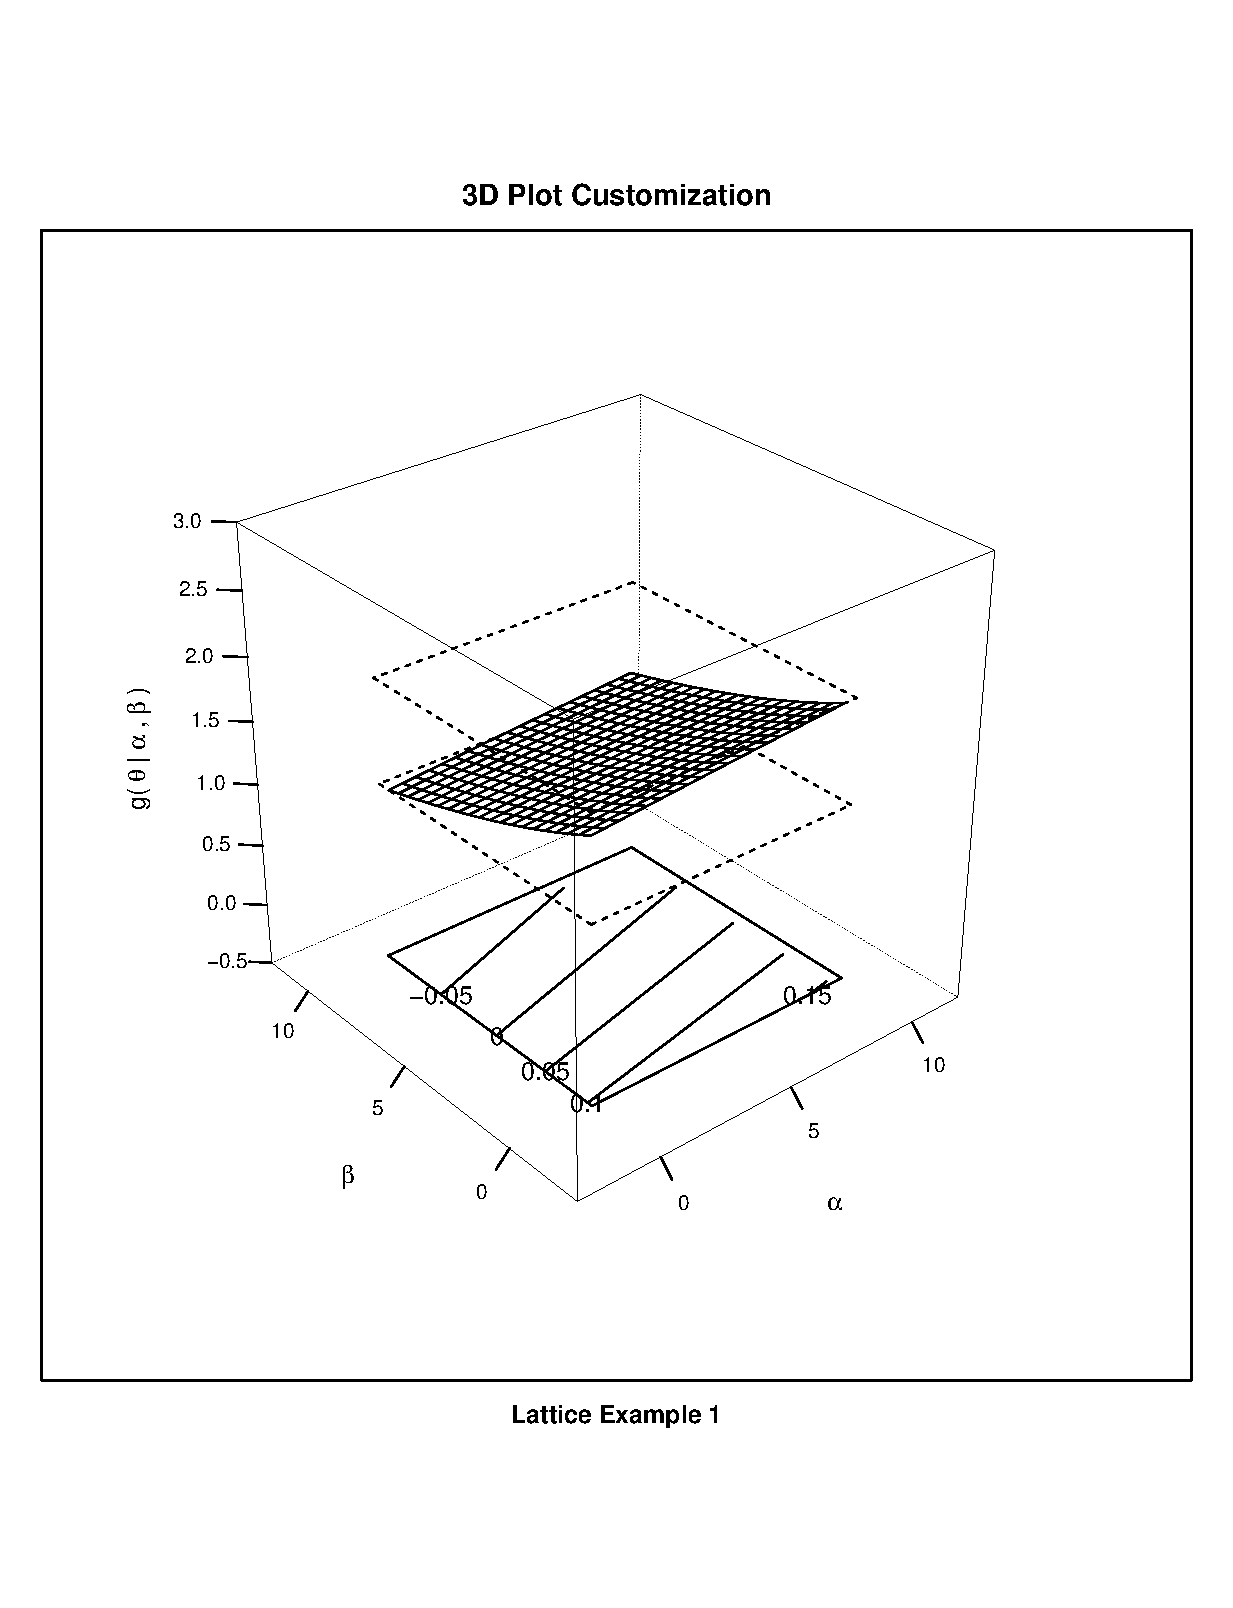
\includegraphics{./img/lattice-fig.eps}


\item \LaTeX 의 문서에 포함될 \texttt{.eps} 그래픽을 \texttt{R}에서 뽑았을 때는 아무런 문제가 없어 보였는데, 정작 \texttt{pdf}로 문서를 뽑아 보니까 이 그래픽이 들어간 페이지가 90도로 돌아가 있거나 혹은 그래픽이 90도로 회전되어 있을 경우에는 아래와 같이 하면 됩니다.

\begin{Schunk}
 \begin{Sinput}
  postscript(file=``filename.eps'', onefile=FALSE, horizontal=FALSE)
 \end{Sinput}
\end{Schunk}

이 문제에 대한 출처는 \texttt{postscript} 도움말입니다.

이문제를 다른 방법으로도 해결할 수 있습니다.  (대충 서너개 더 있음).

\item 새로운 그래픽 객체를 생성하는 방법을 설명해줘서 사용자가 추후에 독립적인 그래픽을 생성할 수 있게 도와주기 


	\item (접수: 2013-APR-23)  저는 다각형을 그리고 싶습니다. 
	
	\textsf{(답변)}  이것은 간단히 2차원-랜덤포인트 생성한 뒤에 \texttt{polygon()} 함수를 써서 보여주면 됨. 

\end{enumerate}

% ggplot2에서 stat_density2d에 오류가 있는것 같습니다. 모든 경우에 NA가 return된다는 보고












